\documentclass[11pt]{article}

\usepackage[margin=1in]{geometry}
\usepackage{graphicx}
\usepackage{subcaption}
\usepackage{amsmath}
\usepackage{amssymb}
\usepackage{float}

\title{RL Lab 3 - Monte Carlo \& Temporal Difference predictions}
\author{Adonis Jamal}
\date{}

\begin{document}
\maketitle

\section{Monte Carlo prediction on blackjack}
\subsection{Monte Carlo prediction}
Can you interpret the 3D value function graph?

\begin{figure}[H]
    \centering
    \begin{minipage}{0.48\textwidth}
        \centering
        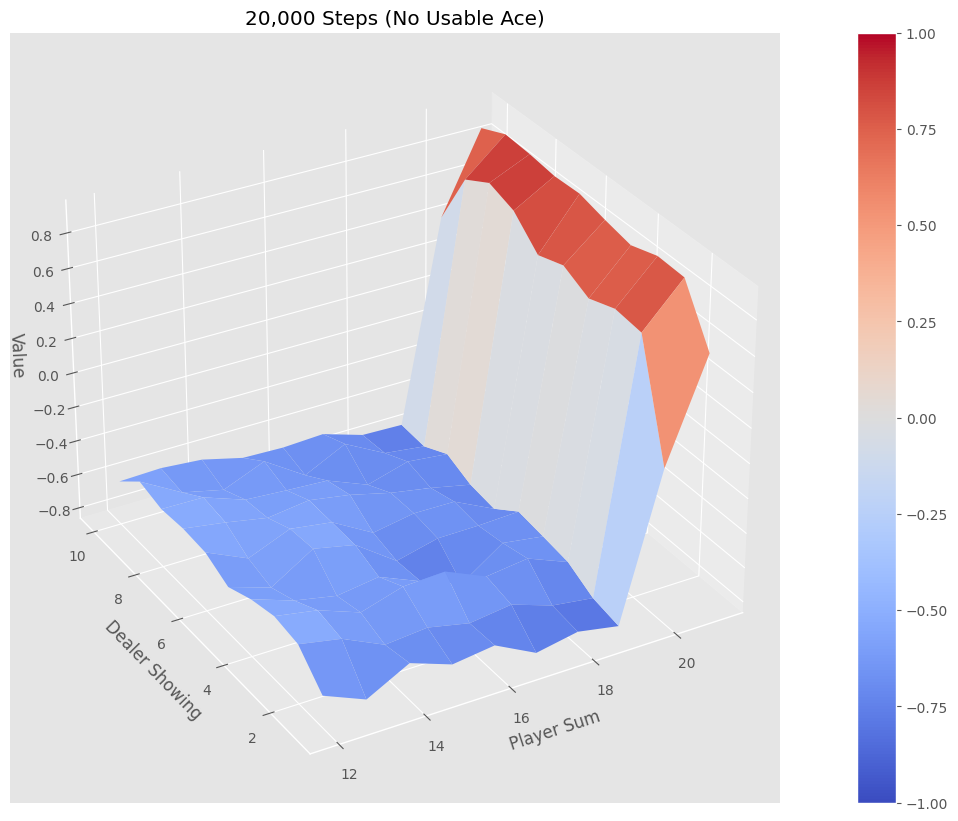
\includegraphics[width=0.48\textwidth]{figures/1.2 MC Prediction No Usable Ace.png}
        \caption{Estimated state-value function without a usable ace.}
        \label{fig:mc_no_usable_ace}
    \end{minipage}
    \hfill
    \begin{minipage}{0.48\textwidth}
        \centering
        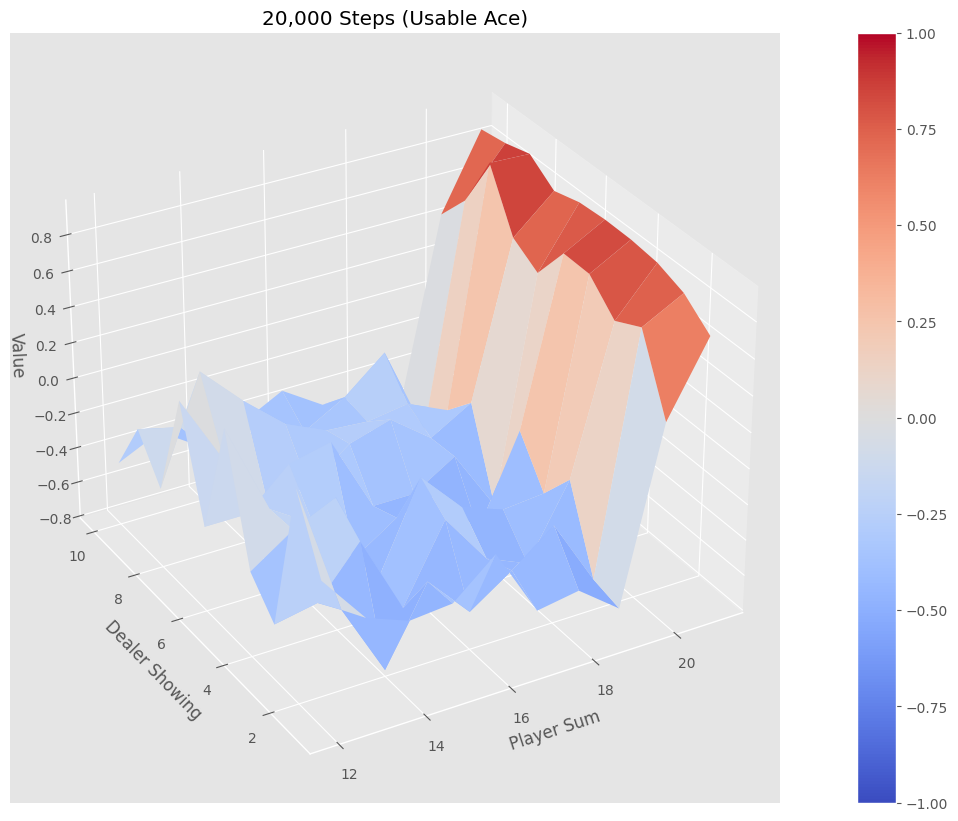
\includegraphics[width=0.48\textwidth]{figures/1.2 MC Prediction Usable Ace.png}
        \caption{Estimated state-value function with a usable ace.}
        \label{fig:mc_usable_ace}
    \end{minipage}
\end{figure}

The graphs (Figures~\ref{fig:mc_no_usable_ace} and~\ref{fig:mc_usable_ace}) illustrate the estimated state-value function for a Blackjack policy where the player hits until they reach a sum of 20 or 21. They show the expected reward based on the player's current sum of cards, and are separated into cases with and without a usable ace. The evaluated policy is highly risky, which is reflected in the steep jump in expected value between sums of 19 and 20. This forces the player to hit on already strong hands like 18 or 19, which frequently results in a bust. On the other hand, the expected value for sums of 20 and 21 is significantly higher, as the player will stick and have a good chance of winning. The presence of a usable ace (Figure~\ref{fig:mc_usable_ace}) also increases the expected value for lower sums, as it provides more flexibility in hitting without busting. Hands drawn with a usable ace occur much less frequently during sampling, leading to a higher variance and less stable value estimates over the same number of episodes.

\subsection{Monte Carlo prediction on multiple episodes}
What's the effect of the number of episodes (num\_episodes) on the learned value function? 

\begin{figure}[H]
    \centering
    % Row 1
    \begin{subfigure}{0.18\textwidth}
        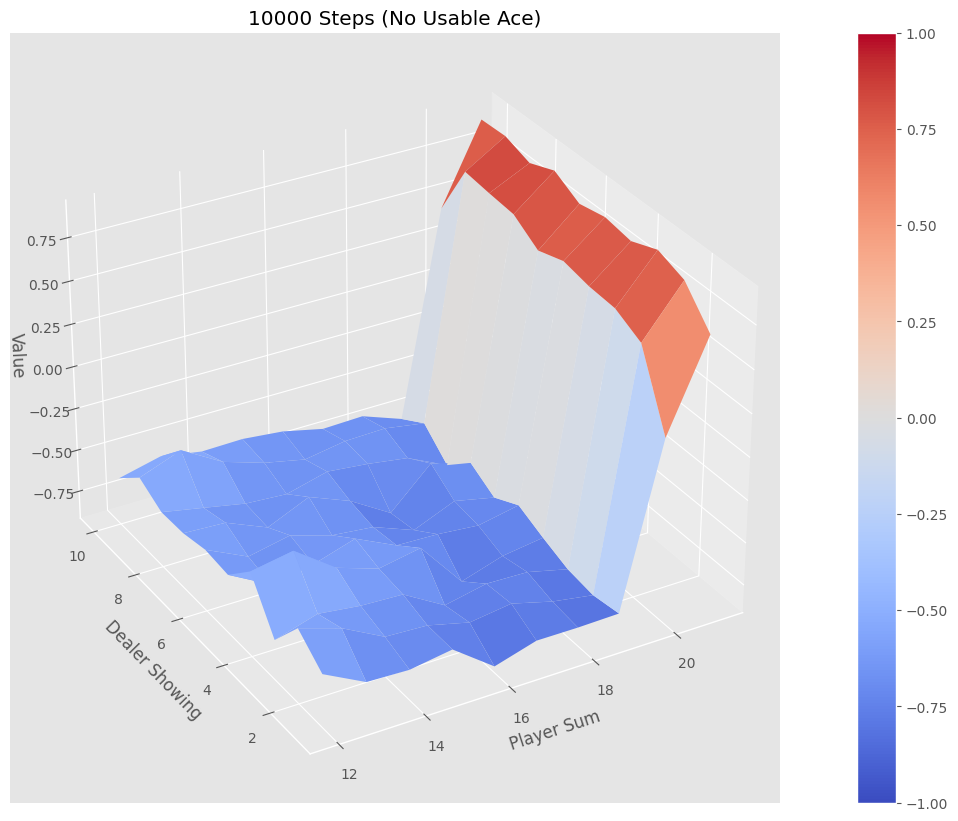
\includegraphics[width=\linewidth]{figures/1.3 10k no ace.png}
        \caption{10k, no usable ace}
    \end{subfigure}
    \hfill
    \begin{subfigure}{0.18\textwidth}
        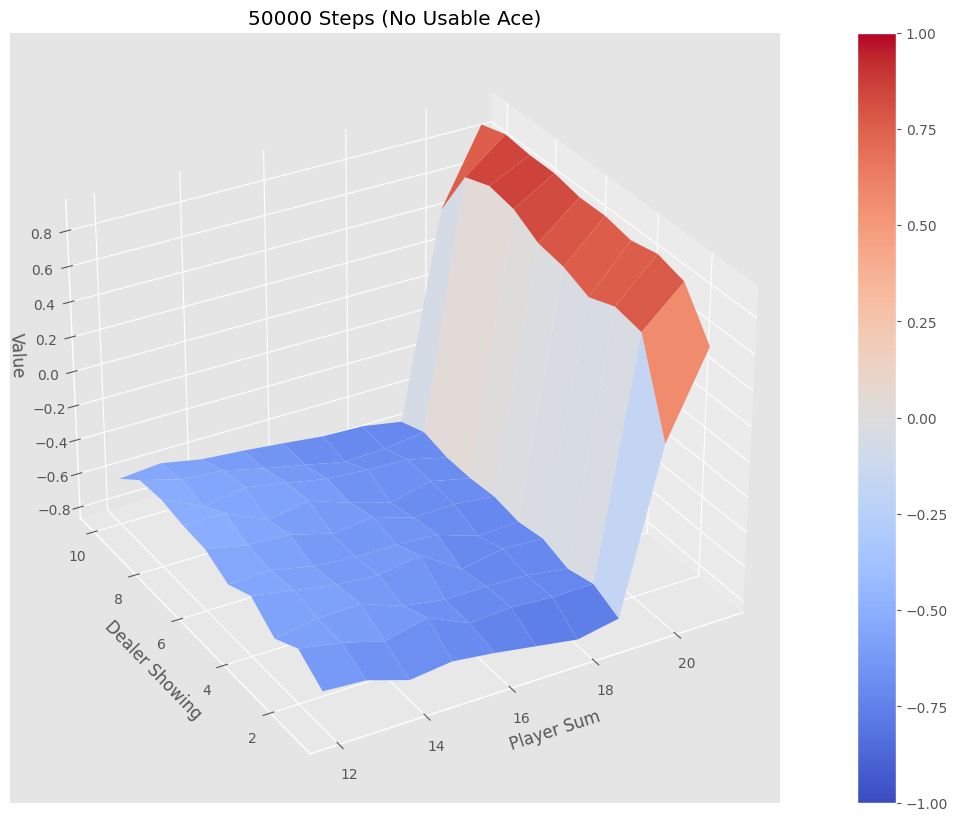
\includegraphics[width=\linewidth]{figures/1.3 50k no ace.png}
        \caption{50k, no usable ace}
    \end{subfigure}
    \hfill
    \begin{subfigure}{0.18\textwidth}
        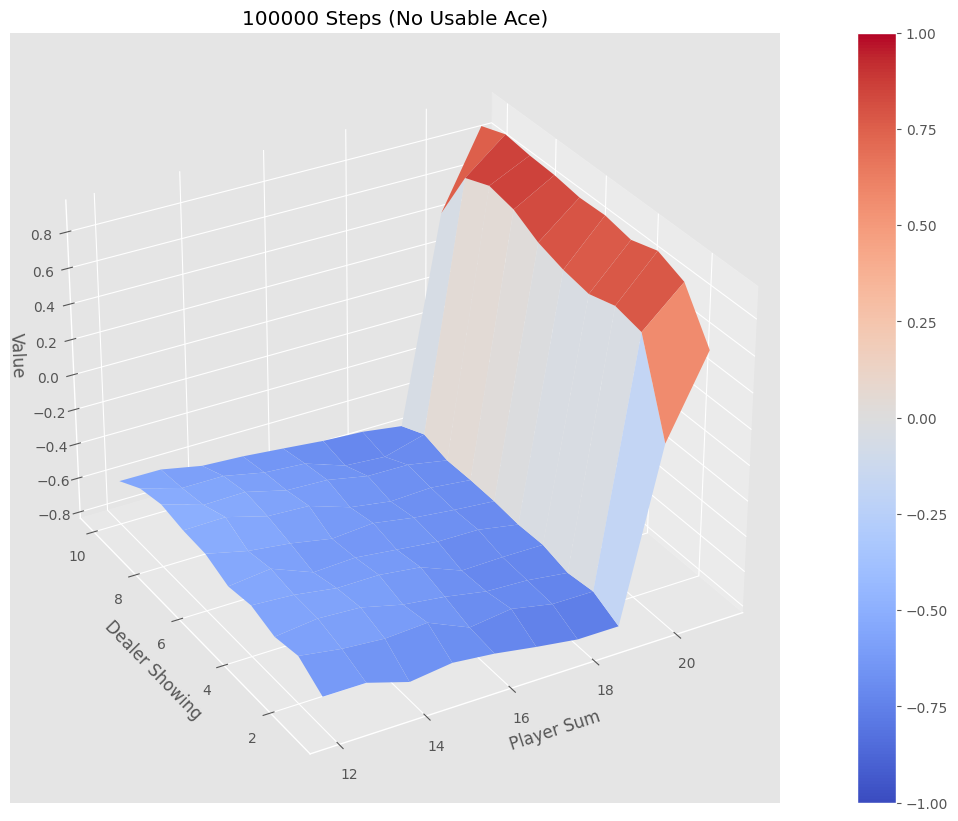
\includegraphics[width=\linewidth]{figures/1.3 100k no ace.png}
        \caption{100k, no usable ace}
    \end{subfigure}
    \hfill
    \begin{subfigure}{0.18\textwidth}
        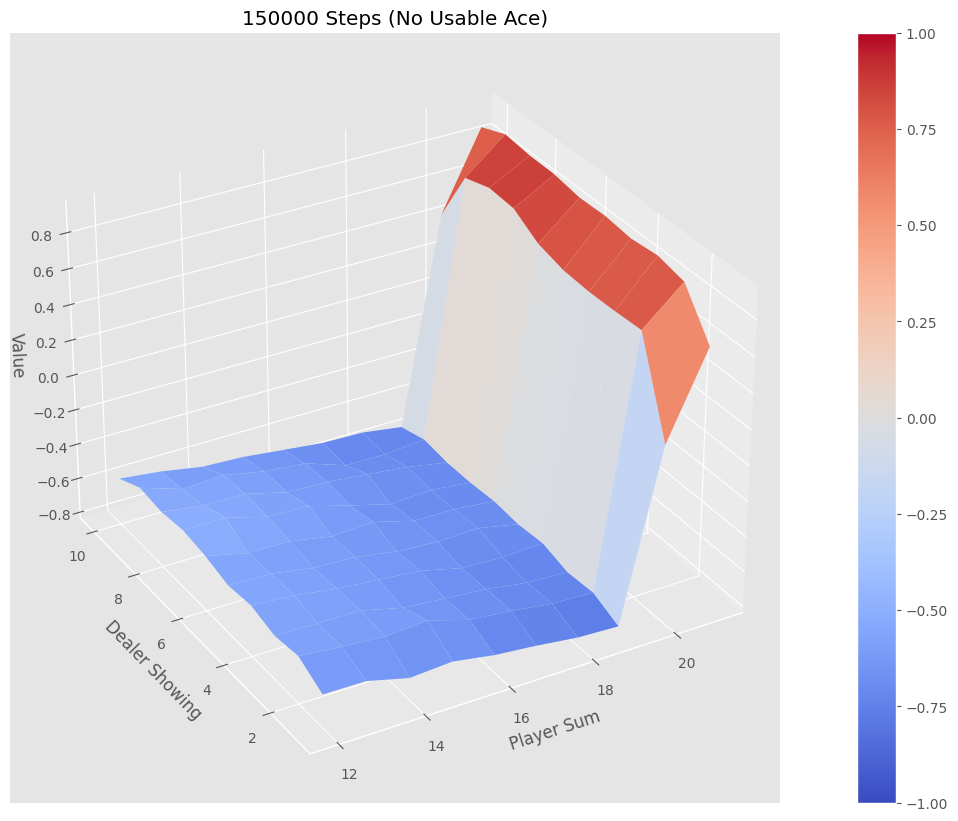
\includegraphics[width=\linewidth]{figures/1.3 150k no ace.png}
        \caption{150k, no usable ace}
    \end{subfigure}
    \hfill
    \begin{subfigure}{0.18\textwidth}
        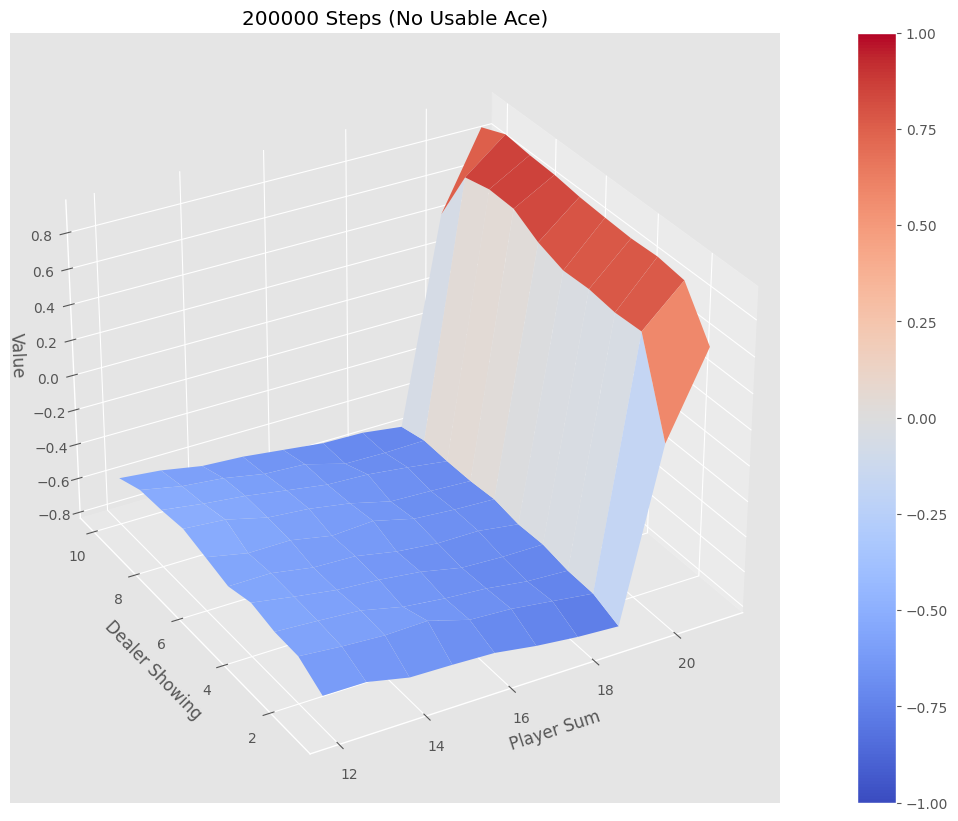
\includegraphics[width=\linewidth]{figures/1.3 200k no ace.png}
        \caption{200k, no usable ace}
    \end{subfigure}

    \vspace{0.5em}

    % Row 2
    \begin{subfigure}{0.18\textwidth}
        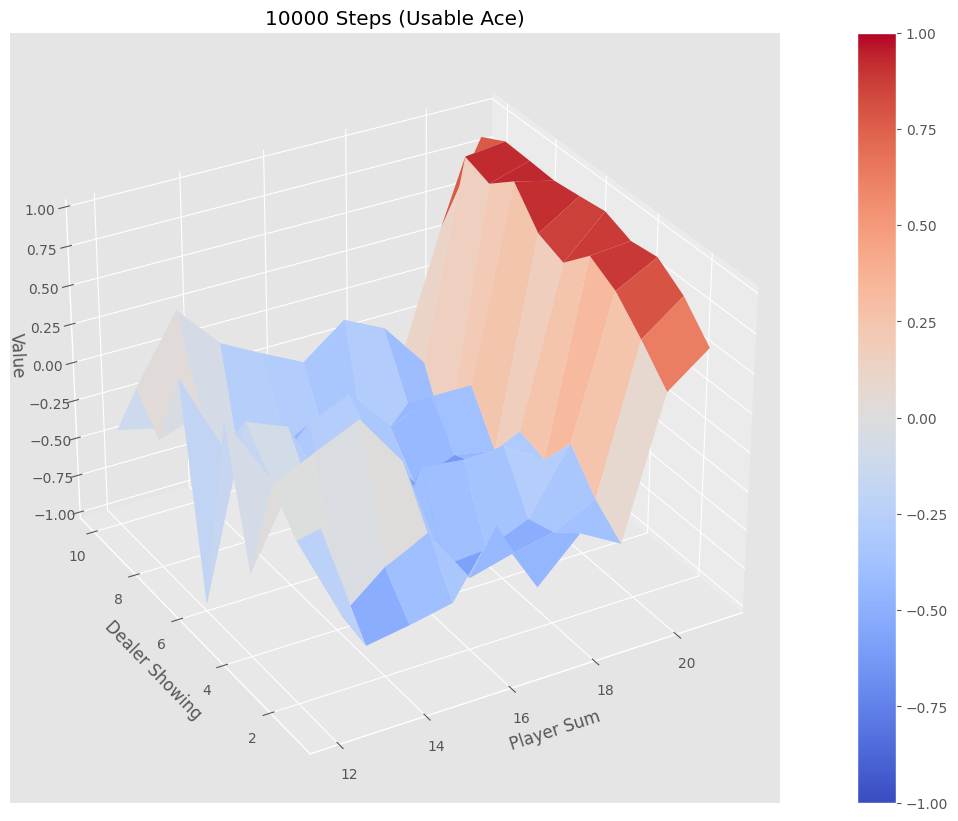
\includegraphics[width=\linewidth]{figures/1.3 10k ace.png}
        \caption{10k, usable ace}
    \end{subfigure}
    \hfill
    \begin{subfigure}{0.18\textwidth}
        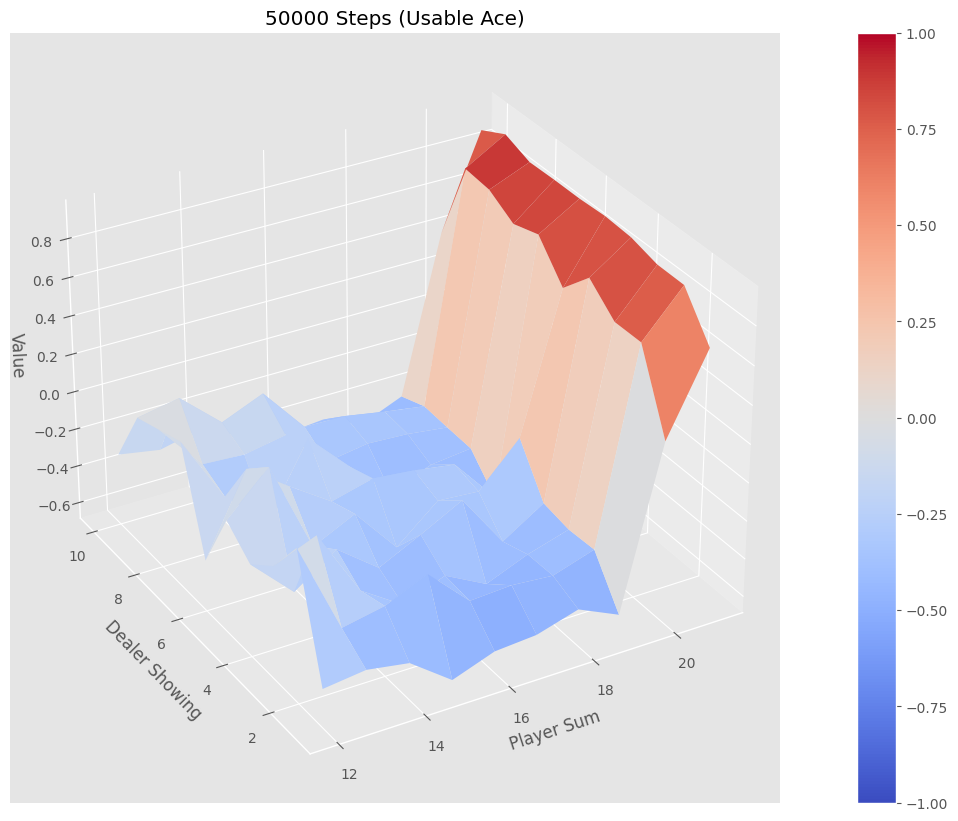
\includegraphics[width=\linewidth]{figures/1.3 50k ace.png}
        \caption{50k, usable ace}
    \end{subfigure}
    \hfill
    \begin{subfigure}{0.18\textwidth}
        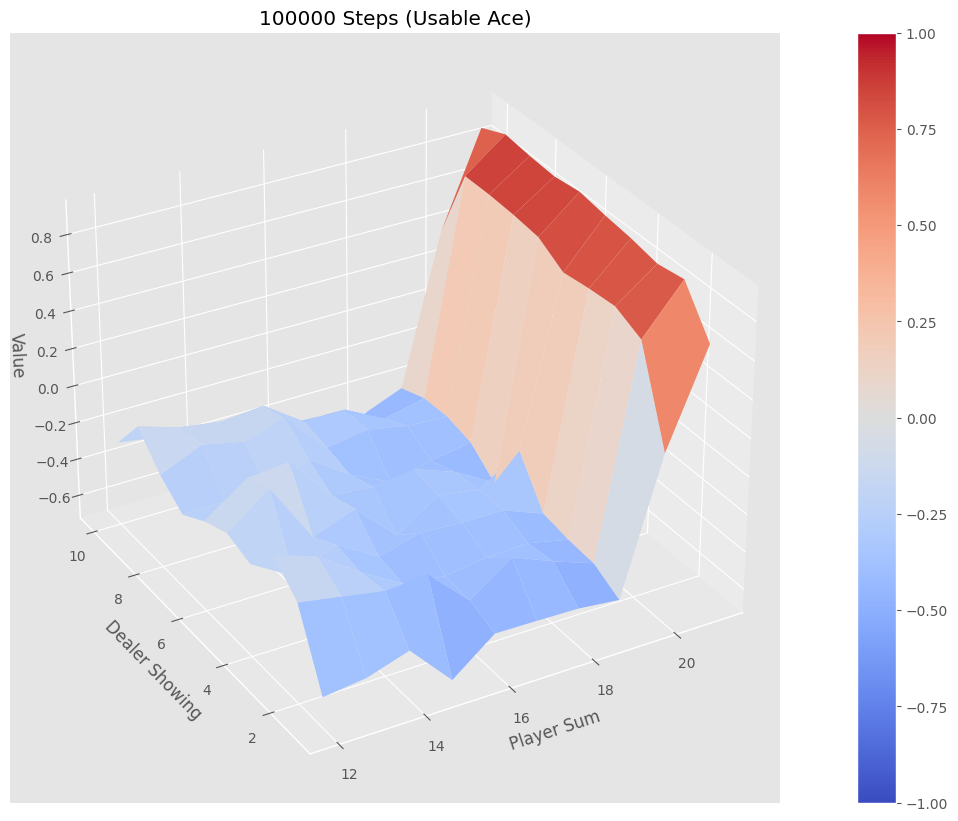
\includegraphics[width=\linewidth]{figures/1.3 100k ace.png}
        \caption{100k, usable ace}
    \end{subfigure}
    \hfill
    \begin{subfigure}{0.18\textwidth}
        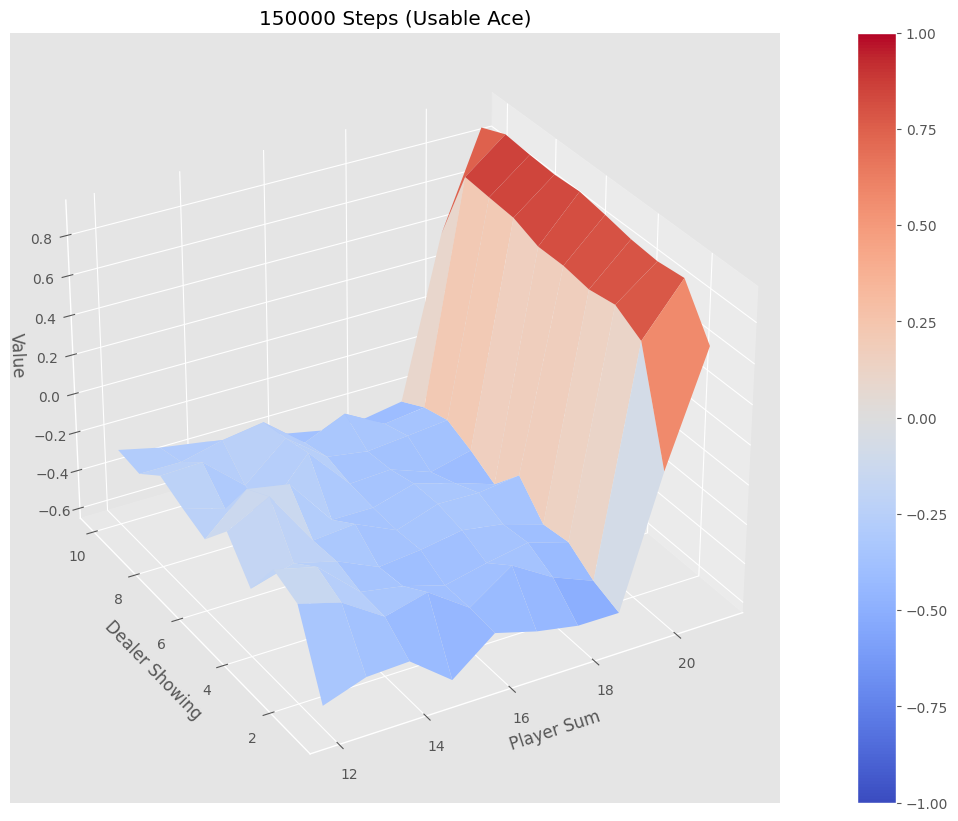
\includegraphics[width=\linewidth]{figures/1.3 150k ace.png}
        \caption{150k, usable ace}
    \end{subfigure}
    \hfill
    \begin{subfigure}{0.18\textwidth}
        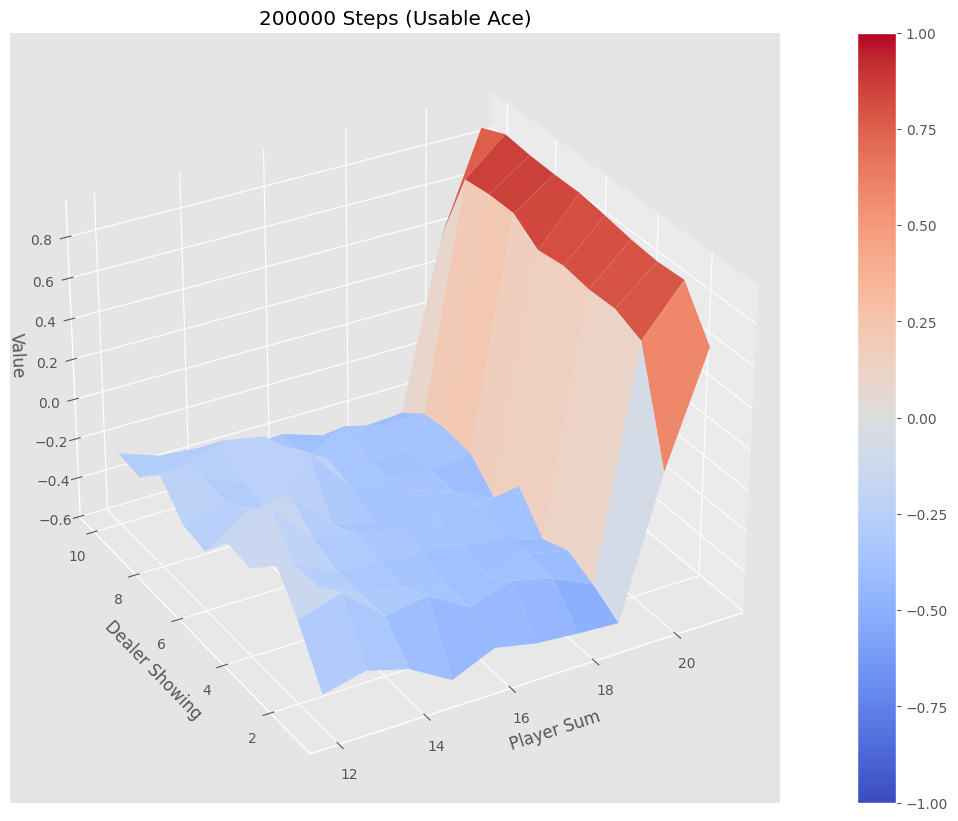
\includegraphics[width=\linewidth]{figures/1.3 200k ace.png}
        \caption{200k, usable ace}
    \end{subfigure}

    \caption{Estimated state-value function for different numbers of episodes, separated by the presence of a usable ace.}
    \label{fig:grid}
\end{figure}

As shown in Figure~\ref{fig:grid}, the number of episodes impacts the accuracy and stability of the learned value function in Monte Carlo prediction. When trained on a smaller number of episodes (such as $10000$), the resulting value function graph appears highly jagged and less smooth, due to the high variance in the estimates. With fewer episodes, many states may not be visited enough times to provide reliable estimates. As the number of episodes increases, the graph becomes smoother and more stable, as the value estimates converge towards their true values. This is due to the law of large numbers. It is important to note that the value function estimates for states with a usable ace are more volatile, as these states are less frequently visited during sampling, leading to higher variance in their estimates, but still benefit from increased episodes for improved accuracy.


\section{Temporal Difference}
\subsection{Comment on the effects of number of episodes on TD's estimated value graph and interpret the results.}

\begin{figure}[H]
    \centering
    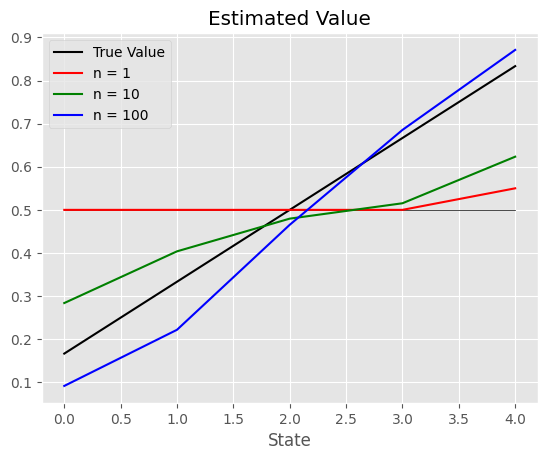
\includegraphics[width=0.8\linewidth]{figures/TD vs MC comparison on RW.png}
    \caption{Temporal Difference (TD) estimated value graph for different numbers of episodes.}
    \label{fig:td_comparison}
\end{figure}

In the initial state ($n=0$), all states are initialized to 0.5. After just one episode, only a few states start to update (Figure~\ref{fig:td_comparison}), while the rest remain stuck at their initial 0.5 guess because TD(0) only looks one step ahead. Over time, as more episodes are played ($n=10$ and $n=100$), the estimates start to converge towards the true value function, which is a straight line from 0 to 1 across the states. This illustrates how TD learning updates its estimates based on the observed rewards and the estimated value of the next state.


\subsection{Empirical RMS error}
Comment on the effects of the step size on the empirical RMS error and explain the results. Compare TD and MC performances and interpret, i.e., give your intuitions as to why one is outperforming the other. 

\begin{figure}
    \centering
    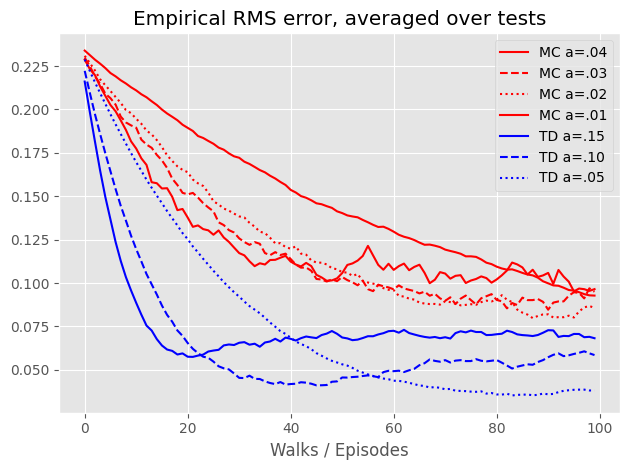
\includegraphics[width=0.8\linewidth]{figures/empirical RMS error.png}
    \caption{Empirical RMS error of TD(0) and Monte Carlo methods for different step sizes $\alpha$ as a function of the number of episodes.}
    \label{fig:rms_error}
\end{figure}


In Figure~\ref{fig:rms_error}, we see the root-mean-squared-error (RMSE) of the value estimates for both TD(0) and Monte Carlo (MC) methods as a function of the number of episodes. 

Larger values of the step size $\alpha$ enable both algorithms to rapidly decrease the empirical RMS error during the first few episodes, but they ultimately lead to higher RMSE values asymptotically because the estimates continuously fluctuate around the true values instead of perfectly converging.

Smaller step sizes result in slower initial learning but eventually settle at a lower, more stable error.

When comparing the two methods, the TD method consistently outperforms MC by achieving a lower RMS error in fewer episodes. This superior performance stems from TD's ability to bootstrap (update its estimates based on the immediate reward and the estimated value of the next state rather than waiting for the episode to finish). By learning from step-to-step transitions and leveraging the Markov property, TD can update its value estimates more efficiently and reduce the high variance associated with MC methods, which rely on complete returns.


\end{document}
